\section{AMIDST Model Class}

\subsection{Introduction  and Notation}

One of the main goals of this project was the definition of a general model class which the following features: (i) it has to be applicable to the three use-cases; (ii) it should be general enough to apply to other future similar use-cases;  (iii) and it should contain certain structure that can be exploited to make this model class valid for scalable inference and learning in massive data streams. 

With these three aims in mind,  we started the definition of the general model class by finding commonalities between the different models presented in Section \ref{Section:PreliminaryModels}.  With this aim, we  introduce some new ``graphical'' notation to ease this process. This new graphical notation is based on the use of subnetworks modules, i.e. some part of the dynamic Bayesian network with some common features such as all the nodes are continuous and observed.  We represent these subnetworks modules by square boxes, in opposite to circle or ellipsed nodes used to represents single variables in a graph. Following a similar notation we used for nodes (see Figure \ref{Figure:PreliminariesNotation}), square boxes rounded by dashed lines refers to a subnetwork which is not observable (i.e. composed by hidden variables); square boxes rounded by continuous lines refers to a subnetwork where the nodes are observed; when the square box is coloured, it means that all the nodes of the subnetwork are discrete (green color) or continuous (blue color). Square boxes can also be nested to represent smaller subcomponents inside a bigger subcomponent. In Figure \ref{Figure:ModelClass:Notation} we give a visual description of this notation. 

\begin{figure}
\begin{center}
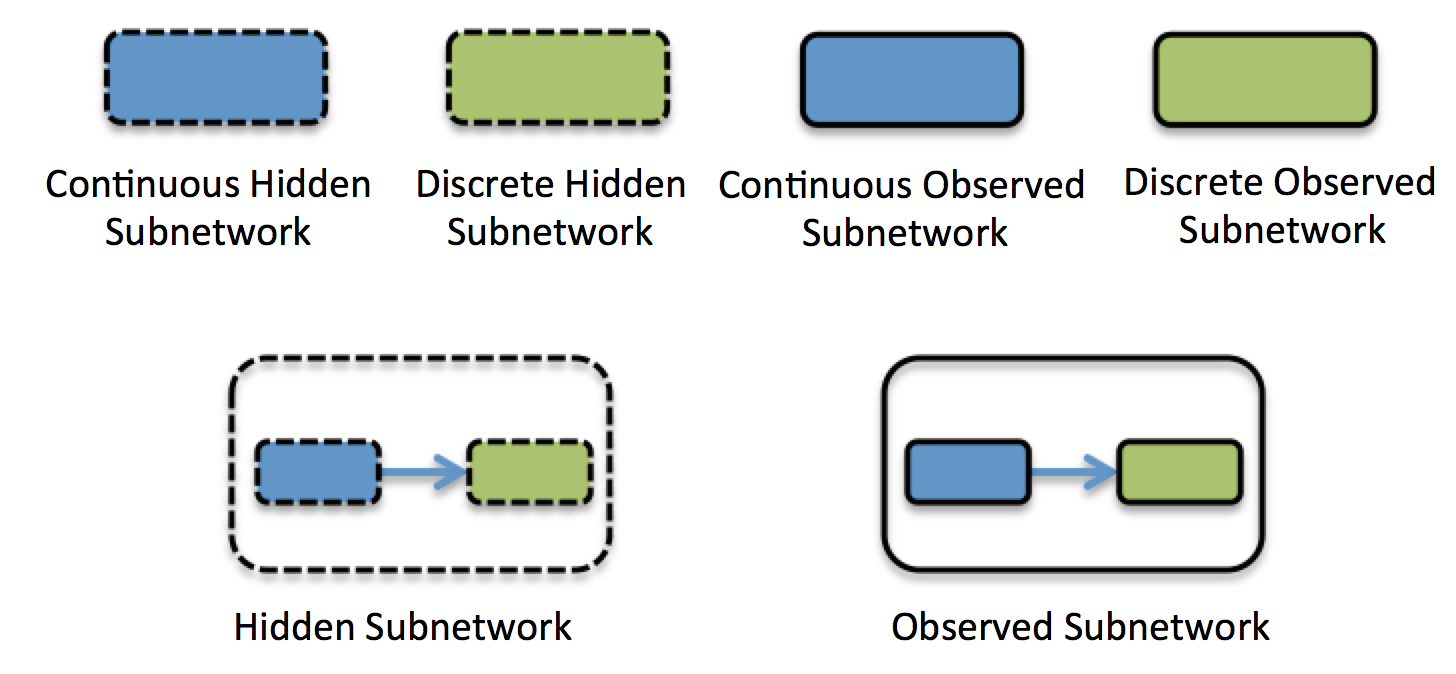
\includegraphics[scale=0.4]{./figures/ModelClass0}
\caption{\label{Figure:ModelClass:Notation} Graphical Notation}
\end{center}
\end{figure}

We present now the models of the three use-cases but using this previously introduced notation. This reinterpretation of the models presented in Section \ref{Section:PreliminaryModels} using these high-level descriptors is made in order to identify the commonalities between all the presented models. 

\subsubsection*{Daimler Model Class}

Daimler's model were visually described in Figures \ref{Figure:daimlerLEdynGeneric}  and \ref{Figure:daimlerreldyn}. As commented in Section \ref{Section:DaimlerDynamic}, one the main issues of these current models is that they contain discrete children with continuous parents and do not fall in the conditional linear Gaussian family \cite{nielsen2009bayesian}. We adopt here the same solution pursed in \cite{kasper2012object} which consists on the discretization of these nodes. In that way, the general structure of Daimler's models would be the one plotted in Figure \ref{Figure:DaimlerModelClass}, where do not have any more discrete children with continuous parents which allows for a standard parametrization \cite{nielsen2009bayesian}. 

\begin{figure}
\begin{center}
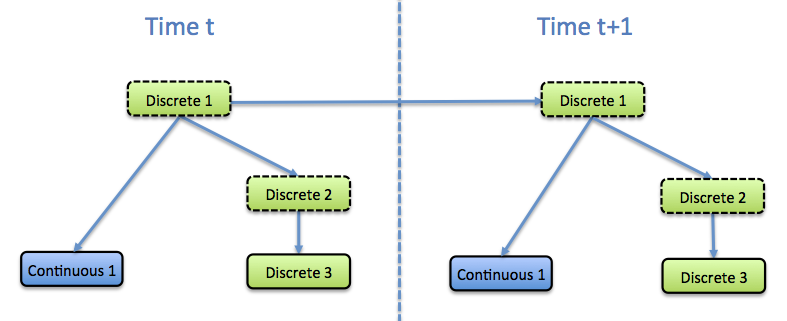
\includegraphics[scale=0.4]{./figures/DaimlerModelClass}
\caption{\label{Figure:DaimlerModelClass} Daimler Model Class}
\end{center}
\end{figure}

This general model is structured as a two-time slices dynamic Bayesian network \cite{nielsen2009bayesian}. The static model which is repeated through the time is composed by three elements: a set of hidden discrete nodes on top; and two observed sub-networks, one continuous and one discrete, which directly depends of the hidden sub-network. This dynamic BN is only temporally connected through the hidden sub-network.  In consequence, the future and past time slices of our dynamic BN are conditionally independent given the hidden sub-network corresponding to the present time. Additionally, inside a time slice, the observed continuous and discrete sub-networks are also conditionally independent given the hidden-subnetwork.

We also have more structure that can be exploited during inference and which is not reflected in this meta-network. Specifically, we have that the hidden and observed sub-networks have a poly-tree structure \cite{nielsen2009bayesian}. Then, the static BN as well as the dynamic BN both have poly-tree structure and this can be exploited during inference. 



\subsubsection*{Verdande Model Class}

Verdande's models were visually described in Figures ?, ? and ? for the three application scenerios of the Verdande use-case (see Section \ref{Section:VerdandeModels}).
Figure \ref{Figure:VerdandeModelClass} visually describes the high-level model that subsumes the models
of the three application scenarios. If we keep the subnetworks ``Discrete 2'', ``Continuous 1'' and ``Continuous 2'' we have the switching Kalman filter model of application scenario 1 (see Section ?). If we keep ``Continuous 1'', ``Discrete 3'' and ``Continuous 2'' we obtain the model for application scenario 2 (see Section ?). Finally, the model for application scenario 3 is obtained by keeping ``Discrete 1'', ``Discrete 2'' and ``Continuous 2'' (see Section ?).  

\begin{figure}
\begin{center}
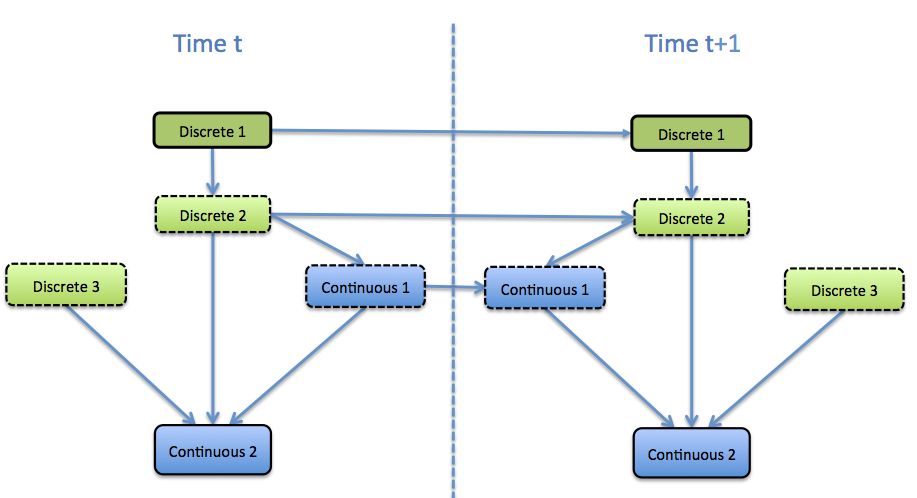
\includegraphics[scale=0.4]{./figures/VerdandeModelClass}
\caption{\label{Figure:VerdandeModelClass} Verdande Model Class}
\end{center}
\end{figure}

Similarly to the Daimler model, the general model is structured as a two-time slices dynamic Bayesian network \cite{nielsen2009bayesian}. The static part which is repeated through the time is composed by 5 sub-networks: two observed components, one discrete temporally connected on the top and one continuous at the bottom; and three hidden components in the middle, one hidden discrete and one hidden continuous temporally connected, and one hidden discrete which is not temporally connected whose function is to account for the possible conditional dependencies of the observed continuous variables.  

In opposite to Daimler,  this model does not have a poly-tree structure that can be exploited during inference. 

\subsubsection*{Caja Mar Model Class}

%\begin{figure}
%\begin{center}
%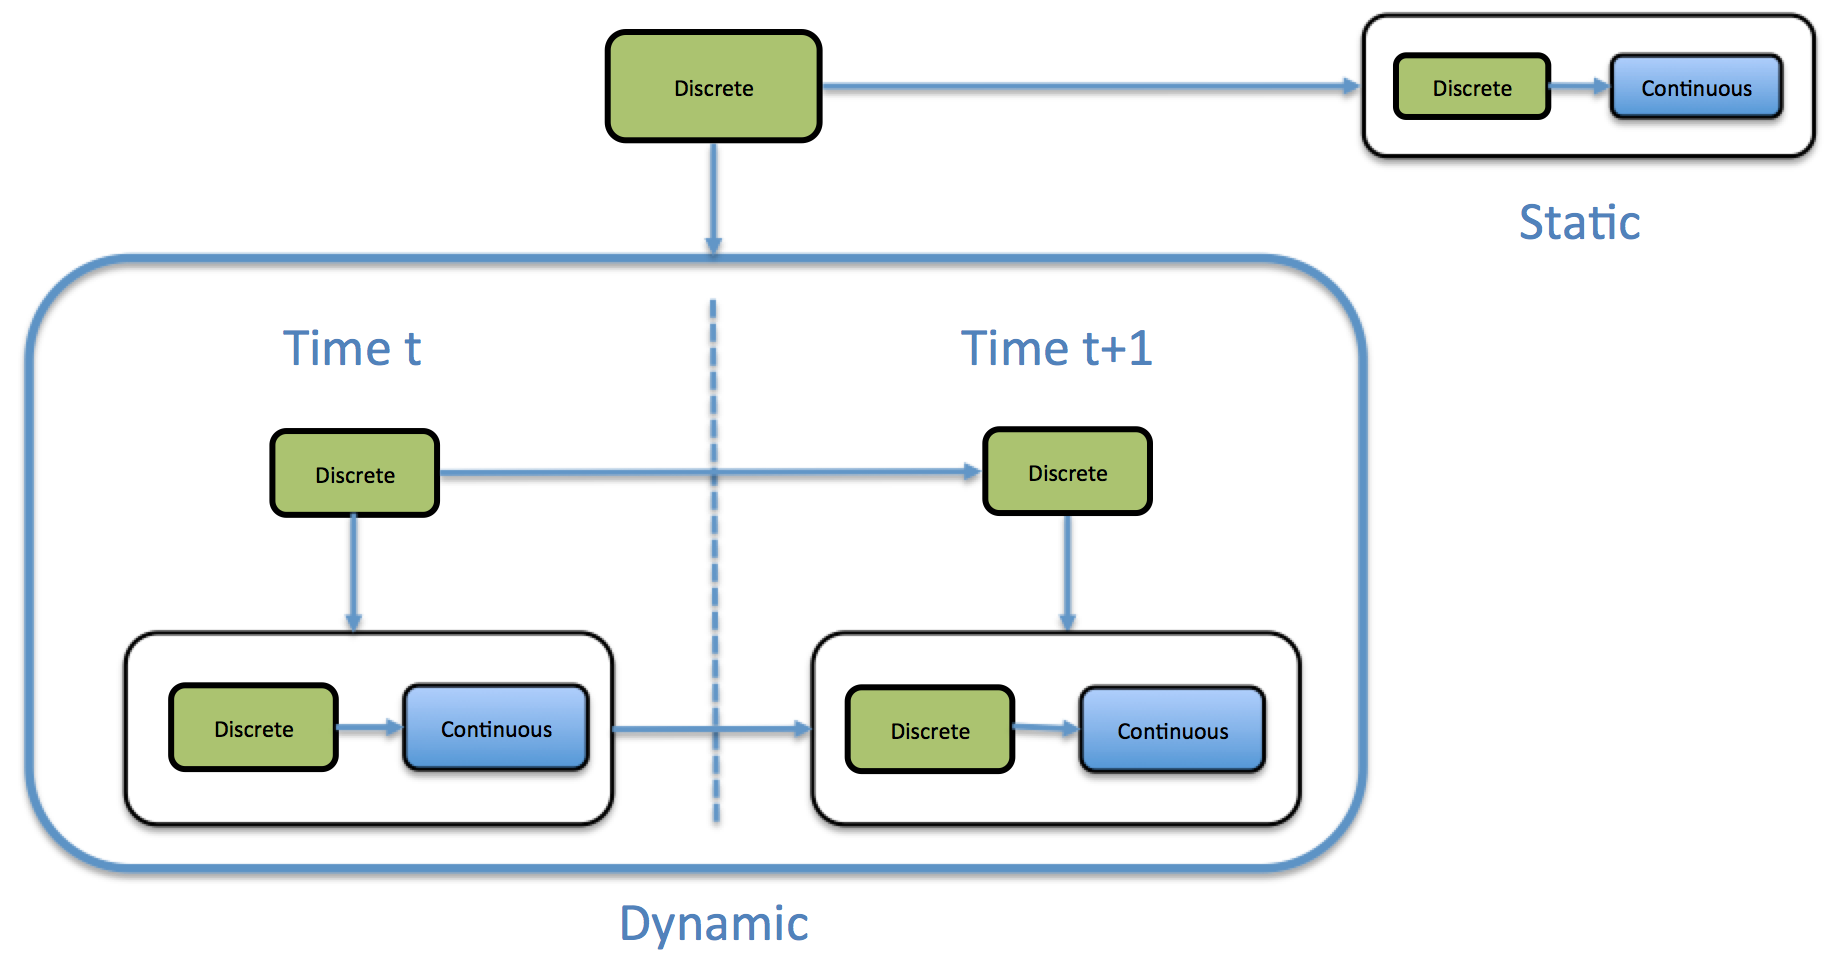
\includegraphics[scale=0.4]{./figures/CajaMarModelClass}
%\caption{\label{Figure:CajaMarModelClass} CajaMar Model Class}
%\end{center}
%\end{figure}



\subsection{AMIDST Model Class}




%\begin{figure}
%\begin{center}
%\caption{\label{Figure:AMIDSTModelClass} CajaMar Model Class}
%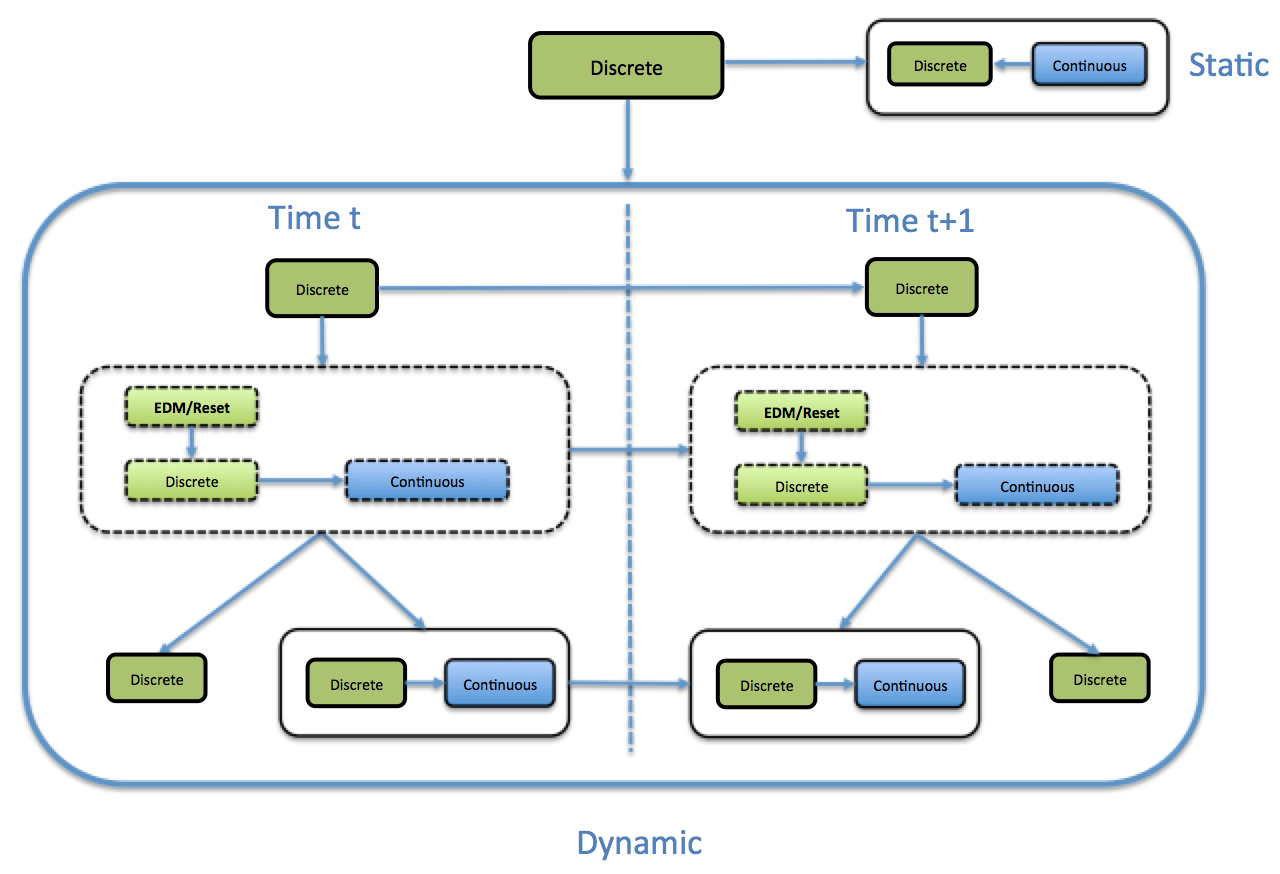
\includegraphics[scale=0.7]{./figures/AMIDSTModelClass}
%\end{center}
%\end{figure}